\section {Case Studies}

It is probably best to consider this section as a series of case
studies of normalization and generalization, rather than a complete
experimental evaluation.  We believe these examples make it clear that
our current algorithms are practically useful, and merit further
development and optimization.

\subsection{AVLTree}

For basic experiments on the ability of normalization to reduce the
number of failing test cases and preserve fault detection, we used a
simple Python implementation of AVL trees found on the web
\cite{avltree}, with 225 lines of code.

\begin{figure}
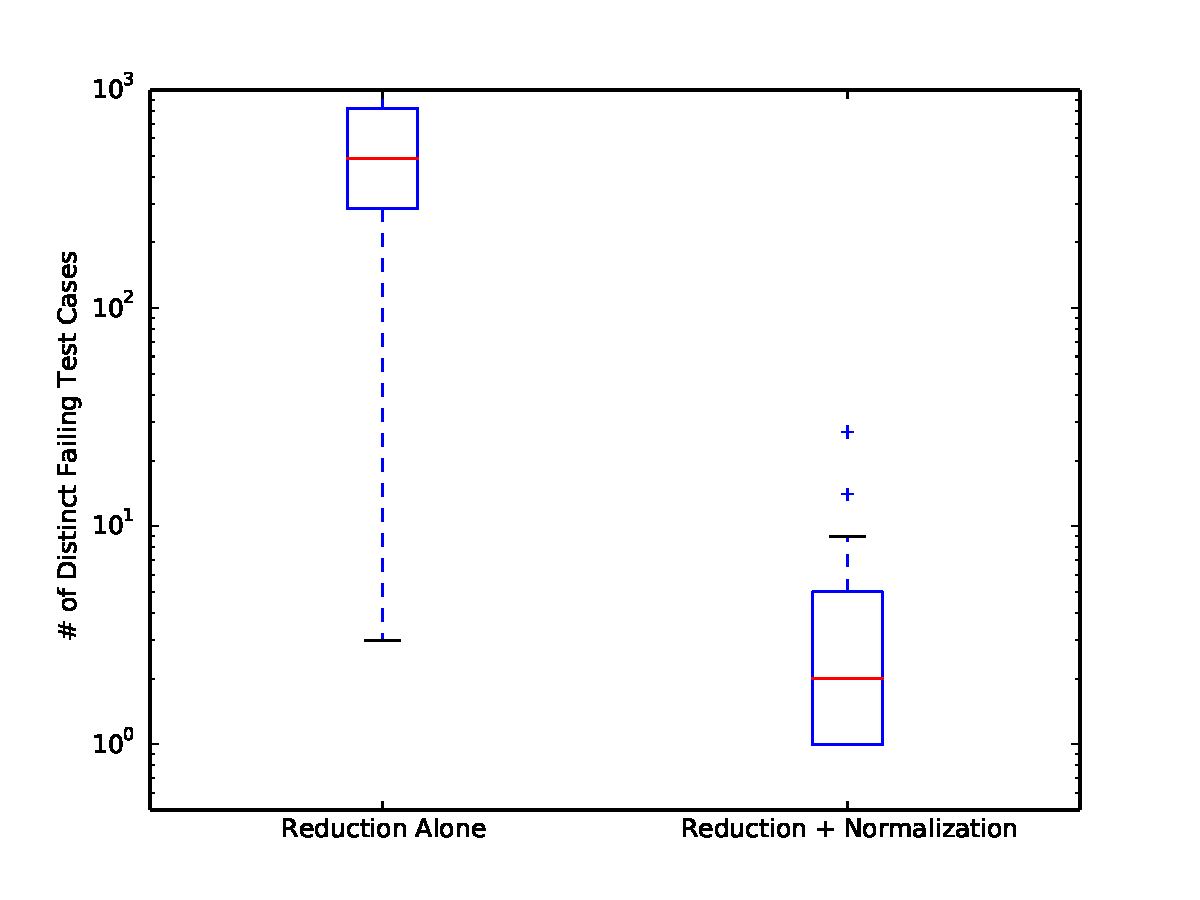
\includegraphics[width=\columnwidth]{length}
\caption{Effects of normalization on 82 AVL Tree mutants.}
\label{normeffect}
\end{figure}

Figure \ref{normeffect} shows the reduction in number of distinct
failing test cases produced by normalization (vs. reduction only) for
a set of 82 mutants of the AVLTree source code\footnote{All graphs
  produced using matplotlib \cite{Hunter:2007}.}.  Of the 228 mutants
produced by MutPy \cite{mutpy}, only these produced at least 1 failure
in 1,000 test cases.  Using only delta-debugging-based reduction, the
mean number of distinct failures for each mutant (which is, by nature,
a single fault) was 498.4, with a median of 485.  Using normalization,
the mean was 3.1 distinct failures, with a mean of just 2 failures.
For 38 of the 82 mutants, normalization produced only a single
representative failure.  For every mutant, normalization reduced the
number of distinct failures, and no mutant produced more than 27
distinct failures, after normalization.

\subsection{XML Parser}

We also examined how normalization combined with multiple faults for a
simple XML parser with about 260 lines of code \cite{myxml}, with one
original fault (a crash instead of a parse error when given an empty
tag ({\tt <>}) and one seeded fault (failure when adding two nodes
with the same name).  Running 1,000 tests produces 848 failing test
cases.  Without normalization, it takes only 37.45 seconds to execute
all 1,000 tests, including delta-debugging these 848 failures.
However, the output is 717 distinct failing test cases.  Normalizing
increases the runtime to 354.7 seconds, but reduces the number of
distinct failing tests to 5, with 3 variations of the original fault
and 2 variations of the seeded fault.  Generalizing these 5 failures
increases the runtime by less than 5 seconds.

\subsection{TSTL}

\subsection{NumPy}

NumPy \cite{NumPy} is a very widely used Python library/extension that supports
large, multi-dimensional matrices and provides a huge library of
mathematical functions.  The popular SciPy library for scientific
computing builds on NumPy.  Developing tests for NumPy is challenging,
because none of the authors are experts in numeric computation, and
the specification of correct behavior is often somewhat subtle.  As a
simple example, consider the test case in Figure \ref{numpyorig},
normalized and generalized in Figure \ref{numpynormgen}.  Prior to
normalization, understanding why the test case leads to a violation of
self-equality for an array is, to say the least, non-trivial.  After
normalization, it is much clearer what is happening:
1) {\tt array0} contains {\tt NaN} 2) this is in fact correct
behavior (the array \emph{should} contain {\tt NaN}).  The greater
length and much larger number of operations involved in the original
reduced test case obscures this critical point.  In NumPy, array
equality does not hold for objects containing {\tt NaN}, so the
assertion must be modified to exclude this case.

Other, more complex, cases have also made it clear that normalization
is useful for some additional test case reduction and generalization
makes any surprising restrictions on test values clear.  For NumPy
tests, normalization takes considerably longer than reduction, in part
due to the expense of operations on large arrays.  Over almost all
examples, the average time to reduce tests is about 4-5 seconds, and
the time for normalization is between 712 and 774 seconds.  The
average time to discover a failing test case, for comparison, is just
over 400 seconds.  Generalization takes between 52 and 59 seconds in
these cases.  The exception was a test case of 45,206 steps (!)
leading to a memory exhaustion error and crash, reduced (over a period
of nearly a day) to a test case with 10 steps, which then normalized
(in only 2 hours) to a test case with 8 steps, involving no operations
other than array initialization (with zeros or ones), array
flattening, and array addition (the original test case involved larger
dimensions, array multiplication, and array subtraction).  This is the
only case in which we have seen normalization time lower than
reduction time.

\begin{figure}
{\scriptsize
\begin{code}
 dim1 = 1 
 shape2 = (dim1, dim1, dim1) 
 array1 = np.ones(shape2) 
 array0 = array1 * array1 
 array1 = array1 + array1 
 array4 = array0 + array1 
 array0 = np.reshape(array4,shape2) 
 array3 = array1 * array4 
 array2 = np.ravel(array4) 
 array5 = array2 - array3 
 array4 = array5 * array2 
 array1 = np.unique(array0) 
 array5 = array5 * array3 
 array0 = array1 * array5 
 array5 = np.unique(array0) 
 array1 = array4 - array2 
 array2 = array0.flatten() 
 array0 = array5 + array5 
 array5 = array5 + array2 
 array2 = array0 * array2 
 np.copyto(array5,array2) 
 array2 = array2 * array5 
 array3 = array0 * array2 
 array0 = array3 - array1 
 array4 = array3 * array0 
 array1 = array5 + array4 
 array5 = array0 * array1 
 array0 = array5 - array1 
 array4 = array0 * array3 
 array3 = array4 * array0 
 array1 = array5 + array3 
 array0 = array2 + array1 
 array5 = array5 - array0 
 array5 = array3 * array5 
 array0 = array1 + array5 
 array2 = array3 - array0 
 array4 = array2 * array1 
 array3 = array4 * array2 
 array2 = array0 - array0 
 np.copyto(array1,array3) 
 array4 = array2.flatten() 
 array1 = array1 * array4
 assert (np.array\_equal(array1,array1))
\end{code}
}
\caption{Original ``failing'' test case for numpy (42 steps)}
\label{numpyorig}
\end{figure}

\begin{figure}
{\scriptsize
\begin{code}
dim0 = 1                            \textcolor{black!45}{\# STEP 0}
\textcolor{black!45}{\#  or dim0 = 10 }
shape0 = (dim0)                     \textcolor{black!45}{\# STEP 1}
\textcolor{black!45}{\#  or shape0 = (dim0, dim0) }
\textcolor{black!45}{\#  or shape0 = (dim0, dim0, dim0) }
array0 = np.ones(shape0)            \textcolor{black!45}{\# STEP 2}
array0 = array0 + array0            \textcolor{black!45}{\# STEP 3}
array0 = array0 + array0            \textcolor{black!45}{\# STEP 4}
\textcolor{black!45}{\#  or array0 = array0 * array0 }
array0 = array0 * array0            \textcolor{black!45}{\# STEP 5}
array0 = array0 * array0            \textcolor{black!45}{\# STEP 6}
array0 = array0 * array0            \textcolor{black!45}{\# STEP 7}
array0 = array0 * array0            \textcolor{black!45}{\# STEP 8}
array0 = array0 * array0            \textcolor{black!45}{\# STEP 9}
array0 = array0 * array0            \textcolor{black!45}{\# STEP 10}
array0 = array0 * array0            \textcolor{black!45}{\# STEP 11}
array0 = array0 * array0            \textcolor{black!45}{\# STEP 12}
array0 = array0 * array0            \textcolor{black!45}{\# STEP 13}
array0 = array0 - array0            \textcolor{black!45}{\# STEP 14}
assert (np.array\_equal(array0,array0))
\end{code}
}
\caption{Normalized and generalized test case for numpy (15 steps)}
\label{numpynormgen}
\end{figure}

\subsection{Esri ArcPy}

Esri (the Environmental Systems Research Institute) is the single
largest Geographic Information System (GIS) software vendor, with about 40\%
of global market share.  Esri's ArcGIS tools are extremely widely
used for GIS analysis, in government, scientific research, commercial
enterprises, and education.  Automation of complex GIS analysis and
data management is a frequent need, and Esri has long provided tools
for programming their GIS software tools.  The current method of
choice is a Python site-package, ArcPy \cite{ArcPy}.  ArcPy is a complex library,
with dozens of classes and hundreds of functions distributed over
a variety of of toolboxes.  Most of the code involved in ArcPy
functionality is C++ for which source is unavailable (the source for
the actual ArcGIS tools); the Python source alone is over 70,000 lines
of code.

In order to improve the reliability of ArcPy, we have been
implementing a TSTL-based framework for testing ArcPy itself as well
as libraries based on ArcPy.  The TSTL definition is already more than
twice as large as the next-largest example previously studied, even
though it only includes a small portion of ArcGIS so far. The first
stage of testing has resulted in discovery of several faults in
ArcPy/ArcGIS, some of which not only cause incorrect behavior but
cause a crash that also ends testing.  Before proceeding to more
nuanced testing, it is critical to understand these faults, the set of
behaviors that trigger them, and modify the test definition to avoid
triggering these behaviors with minimal limitations on the thoroughness
of testing.

There is no space in this paper to elaborate on the details of
this large test effort (which has required adding numerous additional
features and modes to TSTL), but normalization and generalization have been very useful in
this process.  Figures \ref{esriorig} and \ref{esrinormgen} show one
crash-inducing test case, after initial delta-debugging (from over
2,000 test steps) (Figure \ref{esriorig}) and with normalization and
generalization (Figure \ref{esrinormgen}).  First, in this setting
normalization has thus contributed a surprising amount of additional
reduction over delta-debugging.  In this example, normalization
reduced the length from 19 steps to 11 steps; in another case, it
reduced the test case from 18 to 14 steps, and in the other crash
fault, it reduced the test case from 27 to 20 steps.  The cost of
normalization is high --- in our runs, it has taken from 17,340
seconds up to 24,769 seconds.  However, in this setting even
delta-debugging is extremely expensive --- the cost of reduction alone
has ranged from 7,930 seconds to 8,688 seconds.  Generalization has
taken from under an hour (3,203 seconds) up to 11,149 seconds.  These
costs are due in part to the need to run tests in a sandbox
environment to avoid killing the Python testing process, and in part
due to the cost of running complex GIS analyses.  However, even with
this high cost, reducing, normalizing, and generalizing test cases has
been a more effective use of our time than trying to understand the
faults without these aids.  For example, in the test case shown in
this paper, it was essential to understand that the SQL query and
selection type were not essential to the fault, but that using a
freshly created layer would not result in a crash:  the problem
appears to be that ArcGIS (or ArcPy) does not invalidate layers built
from a feature class when that feature class is deleted\footnote{In
  this instance, a generalization (the fresh values generalization in
  particular) is informative even though it does not allow any
  generalization; knowing that it was attempted, but prevented the
  failure, is also valuable.}.  The
original, non-normalized test case makes this far less clear, as the
use of {\tt CopyFeatures} and the multiplicity of shapefiles involved
disguises the essence of the problem.

In addition to helping us understand failures, normalization and
generalization are also being used to prepare an API-behavior
regression suite for ArcPy.  One of the challenges of using a large
API like ArcPy is that behavior of the system can change from version
to version; in some cases this is due to new faults, or fixed faults,
but in other cases there is simply an undocumented change.  In order
to assist ArcPy developers, we are preparing a test suite that covers
as much as possible of the Python source for ArcPy, in the latest version of ArcPy,
10.3, and records the values returned in 10.3.  For future versions of
ArcPy (or older versions), a ``semantic diff'' with 10.3, based on
these calls, can be produced by running this suite.  The tests in the
suite are normalized and generalized to help users understand the
conditions behind an API usage's behavior, not just one set of
values.  This ``coverage regression'' quick test \cite{icst2014} may
also be useful for helping users understand the API, since the set of
online examples of usage from Esri is usually limited to a small set
of parameter combinations.

\begin{figure}
{\scriptsize 
\begin{code}
shapefile2 = "C:\\arctmp\\new3.shp" 
shapefile1 = "C:\\arctmp\\new3.shp" 
featureclass2 = shapefile2 
featureclass0 = shapefile1 
shapefilelist2 = 
   glob.glob("C:\\Arctmp\\*.shp") 
fieldname0 = "newf3" 
shapefile1 = shapefilelist2 [0] 
featureclass1 = shapefile1 
arcpy.CopyFeatures\_management
   (featureclass1,featureclass2) 
op1 = ">" 
newlayer2 = "l2" 
val1 = "100" 
selectiontype2 = "SWITCH\_SELECTION" 
fieldname1 = "newf1" 
arcpy.MakeFeatureLayer\_management
   (featureclass0, newlayer2) 
arcpy.SelectLayerByAttribute\_management
   (newlayer2,selectiontype2,
   ' "'+fieldname0+'" '+op1+val1) 
op0 = ">" 
arcpy.Delete\_management(featureclass2) 
arcpy.SelectLayerByAttribute\_management
   (newlayer2,selectiontype2,
   ' "'+fieldname1+'" '+op0+val1) 
\end{code}
}
\caption{Original test case for ArcPy library (19 steps)}
\label{esriorig}
\end{figure}

\begin{figure}
{\scriptsize 
\begin{code}
shapefilelist0 = 
   glob.glob("C:\\Arctmp\\*.shp")        \textcolor{black!45}{\# STEP 0}
\textcolor{black!45}{\#[}
shapefile0 = shapefilelist0 [0]        \textcolor{black!45}{\# STEP 1}
newlayer0 = "l1"                       \textcolor{black!45}{\# STEP 2}
\textcolor{black!45}{\#  or newlayer0 = "l2" }
\textcolor{black!45}{\#  or newlayer0 = "l3" }
\textcolor{black!45}{\#  swaps with steps 3 4 5 6 7}
\textcolor{black!45}{\#] (steps in [] can be in any order)}
\textcolor{black!45}{\#[}
featureclass0 = shapefile0             \textcolor{black!45}{\# STEP 3}
\textcolor{black!45}{\#  swaps with step 2}
fieldname0 = "newf1"                   \textcolor{black!45}{\# STEP 4}
\textcolor{black!45}{\#  or fieldname0 = "newf2" }
\textcolor{black!45}{\#  or fieldname0 = "newf3" }
\textcolor{black!45}{\#  swaps with steps 2 8}
selectiontype0 = "SWITCH\_SELECTION"    \textcolor{black!45}{\# STEP 5}
\textcolor{black!45}{\#  or selectiontype0 = "NEW\_SELECTION" }
\textcolor{black!45}{\#  or selectiontype0 = "ADD\_TO\_SELECTION" }
\textcolor{black!45}{\#  or selectiontype0 = "REMOVE\_FROM\_SELECTION"}
\textcolor{black!45}{\#  or selectiontype0 = "SUBSET\_SELECTION"}
\textcolor{black!45}{\#  or selectiontype0 = "CLEAR\_SELECTION"   }
\textcolor{black!45}{\#  swaps with steps 2 8}
op0 = ">"                              \textcolor{black!45}{\# STEP 6}
\textcolor{black!45}{\#  or op0 = "<" }
\textcolor{black!45}{\#  swaps with steps 2 8}
val0 = "100"                           \textcolor{black!45}{\# STEP 7}
\textcolor{black!45}{\#  or val0 = "1000" }
\textcolor{black!45}{\#  swaps with steps 2 8}
\textcolor{black!45}{\#] (steps in [] can be in any order)}
arcpy.MakeFeatureLayer\_management
   (featureclass0, newlayer0)          \textcolor{black!45}{\# STEP 8}
\textcolor{black!45}{\#  swaps with steps 4 5 6 7}
arcpy.SelectLayerByAttribute\_management
   (newlayer0,selectiontype0,
   ' "'+fieldname0+'" '+op0+val0)      \textcolor{black!45}{\# STEP 9}
arcpy.Delete\_management(featureclass0) \textcolor{black!45}{\# STEP 10}
arcpy.SelectLayerByAttribute\_management
   (newlayer0,selectiontype0,
   ' "'+ fieldname0+'" '+op0+val0)     \textcolor{black!45}{\# STEP 11}
\end{code}
}
\caption{Normalized and generalized test case for ArcPy library
  (12 steps)}
\label{esrinormgen}
\end{figure}